\documentclass[12pt,a4paper,finnish]{tillbehor/tutthesis}
 
% LaTeX-tiedosto opinnäytepohjaksi
% Tekijä: Sami Paavilainen
% Muokkaaja: Heikki Huttunen (heikki.huttunen@tut.fi) 31.7.2012.
 
% Vaatii lisäksi luokkatiedoston tutthesis.cls
% sekä tiedoston tty-logo.pdf (pdflatex) tai tty-logo-eps (latex)

\usepackage[utf8]{inputenc}

\usepackage[small]{caption}% kuvatekstien kirjasinkoko ja asettelu
%omia käskyjä voi lisätä tähän väliin, esim. \newcommand{\angs}{\textsl{\AA}}
\pagenumbering{Roman}
% alkuvalmistelut loppuu
 
\begin{document}

 
\thispagestyle{empty}
 
\vspace*{-.5cm}\noindent
 
% If thesis is in English, use the file "tut-logo"
% instead of "tty-logo" in the following:
 

\includegraphics[width=8cm]{tillbehor/tut-logo}
 
\vspace{6.8cm}
 
\noindent{\bf\large \textsf{Mikko Pohja}}\\
{\bf\large \textsf{Maximizing quality in a small budget software project}}\\
\textsf{Master of Science Thesis}
 
\vspace{8.7cm} % jos kaksi otsikkoriviä vaihda -> 6.7cm
 
\begin{flushright}
  
\begin{minipage}[c]{6.8cm}
\begin{spacing}{1.0}
\textsf{Examiners: Tarkastaja 1}\\
\textsf{Examiners and topic approved in}\\ 
\textsf{the Information Technology}\\
\textsf{Department Council meeting on}\\
\textsf{xx.xx.xxxx}\\
\end{spacing}
\end{minipage}
\end{flushright}
 
\newpage
 
\setcounter{page}{1} % tämä tarvitaan, jottei ensimmäinen sivu kansilehden jälkeen olisi numero 2.
 
\chapter*{TIIVISTELMÄ}
\begin{spacing}{1.0}
\textsf{TAMPEREEN TEKNILLINEN YLIOPISTO}\\
\textsf{Tietotekniikan koulutusohjelma}\\
{\bf \textsf{Mikko Pohja: Maximizing quality in a small budget software project}}\\
\textsf{Diplomityö, xx sivua, x liitesivua}\\
\textsf{Xxxxxkuu 201x}\\
\textsf{Pääaine: }\\
\textsf{Tarkastajat: }\\
\textsf{Avainsanat: }\\
\end{spacing}
 
\noindent
Ensimmäinen kappale
 
\noindent
Toinen kappale
\newpage
\chapter*{ABSTRACT}
\begin{spacing}{1.0}
\textsf{TAMPERE UNIVERSITY OF TECHNOLOGY}\\
\textsf{Master's Degree Programme in Information Technology}\\
{\bf \textsf{AUTHOR : Title}}\\
\textsf{Master of Science Thesis, xx pages, x Appendix pages}\\
\textsf{xxxxxx 201x}\\
\textsf{Major: }\\
\textsf{Examiner: }\\
\textsf{Keywords: }\\
\end{spacing}
 
\noindent 
First paragraph
 
\noindent
Second paragraph
 
\newpage
 
\chapter*{PREFACE}
\noindent Tämä (\textit{d-tyo.tex}) on \LaTeX-pohja Tampereen teknillisen
yliopiston opinnäytetöitä varten. Samaan pakettiin kuuluu myös
tiedosto \mbox{\textit{tutthesis.cls}}, joka sisältää taittoteknisiä
lisäyksiä \LaTeX:n alkuperäiseen \textit{report.cls}-luokkatiedostoon.
 
Lisäksi otsikkosivua varten tarvitaan tiedosto \textit{tut-logo.xxx}, jonka
tulee sisältää TTY:n logo. Tiedoston tulee
olla joko \textit{.eps}- tai \textit{.pdf}-muodossa riippuen \LaTeX-versiosta.
 
\newpage
\tableofcontents
%\newpage
%\listoffigures
%\listoftables
\newpage
\chapter*{TERMS AND DEFINITIONS}
 
% Näitä ei välttämättä tarvi olla
\begin{termiluettelo}
 
\item [Life cycle] TODO
\item [Function point] TODO
 
\end{termiluettelo} 
 
 
\newpage
\renewcommand{\chaptermark}[1]{\markboth{\thechapter. \ #1}{}}
\renewcommand{\sectionmark}[1]{\markright{}{}}
\lhead{\fancyplain{}{\leftmark}}
 


% Tästä alkaa varsinainen teksti
\pagenumbering{arabic}
 

\chapter{Introduction}

%Konteksti
% Koodauskielien, frameworkkien, ympäristöjen (as a service) kehittyminen ja osaamisen lisääntyminen on tehnyt mahdolliseksi softan tekemisen ilman massiivista budjettia, suurta tiimiä tai pitkää prosessia.
% Lean ja Agile on helpottanut ja nopeuttanut kehitystyötä ja tehnyt mahdolliseksi nopean validoinnin ja julkaisemisen.
% 

Progress in recent history has made developing new products and services in the field of software development increasingly easy. New and improved programming languages and frameworks are introduced constantly. These frameworks provide easy to start platforms for new software development removing the need for excessive planning and understanding of many low-level implementation details. In addition, the need for expensive hardware setup has come obsolete as several instances have appeared offering reasonably priced execution environments as a service. 

These changes in the industry along with the progress in development processes have brought the possibility to create software business closer to every would-be entrepreneur. Developing software with Agile or Lean methodology with modern technologies have lowered the initial time and resources required. Experienced software developers can implement a prototype as fast as in weeks starting from scratch and ending in having a working product publicly available. Attempts to create the next big software product are on a rise as the stories of success spread around the globe.

% TODO: lisää kontekstia?

%Ratkaistava ongelma
% Helppo ja nopea tekeminen johtaa helposti huonoon laatuun sekä budjetin ja aikataulun kasvuun
% 

Since the number of attempts for success are increasing, so is the number of companies succeeding. When a product built with minimum effort starts to prosper, the demand for high quality emerges. As products done by traditional software development are built with large amounts of effort used to improving the quality of the product, modern startup entrepreneurs may become confused when considering the quality of their product. The methods and activities used in traditional software development may seem separate from the rapid development of modern products. In addition, modern software development methodologies focus on different aspects of software quality than in traditional software development.

%"Tässä diplomityössä..."
% Käsitellään perinteisiä laadunvarmistusmenetelmiä sekä niiden tehokkuutta
% Kerrotaan startupista yleisesti sekä sen määritelmästä laadulle
% Kerrotaan perinteisten laadunvarmistusmenetelmien soveltumisesta nykyisiin startupin juttuihin
% Käsitellään esimerkkinä CASE-projekti, joka on pienehkön budjetin projekti startupille

This thesis presents software quality in a startup environment and suggests the activities for improving it. Traditional quality improvement methods are presented and linked to the methods recommended in startup environments. Also a real-life software project for a Finnish startup is presented for illustration purposes. The project, executed in a Finnish software company Futurice, is evaluated by using the data gathered after the project from interviews of the project stakeholders.

%Rakenne luku kerrallaan + sisällön esittely "lause per luku"

The rest of this thesis is organised as follows. Chapter 2 introduces the background by defining software quality and startup environment. Chapter 3 describes the methods and activities improving software quality and divides them in phases of traditional software development. Chapter 4 redefines quality in context of a software startup and describes the methods of quality improvement applicable in startup software development. Chapter 5 presents the execution and phases of the case project and evaluates the quality achieved based on the interviews of the stakeholders.

 
 %%%%%%%%%%%%%%%%%%%%%%%%%%%%%%%%%%%%%%%%%%%%%%%%%%%%%%%%%%%%%%%%%%%%%%%%%%%%%%%%%%%%%%%%%%%%%%%
 % SOFTWARE QUALITY
 %%%%%%%%%%%%%%%%%%%%%%%%%%%%%%%%%%%%%%%%%%%%%%%%%%%%%%%%%%%%%%%%%%%%%%%%%%%%%%%%%%%%%%%%%%%%%%%
 
 
 \chapter{Background}
 
This chapter describes software quality and startup environment. Section~\ref{sec:software_quality} describes software quality in general and the motivation behind improving quality. Section~\ref{sec:startup} explains the context of a startup environment and the phases in the life of a startup.

 \section{Software Quality}

Quality is an attribute of the item in question. It is often described as a combination of qualitative and quantitative attributes. Quality is an ambiguous attribute, because it is subjective and thus differs when viewed from different perspectives. The American Society for Quality has two definitions for technical quality: 1. the product's ability to satisfy its needs; 2. the product's lack of deficiencies~\cite{ASQglossary}. Software is one of the most used types of product in human history. At the same time it has one of the highest failure rates of any type of products mainly due to poor quality. With those facts, it is clear that the total influence of low quality software is considerable in both money and time. Still it is a known fact that a common practice to cut costs is reducing the effort used in software quality. Convincing the payer to allow using effort to achieve good quality can be difficult but crucial. The topic is widely researched and the results speak on behalf of quality.

TODO: Tästä pitäisi johdatella seuraavaan sisältöön

\subsection{Motivation}

Phil Crosby has made popular a concept that establishing a quality program will return in savings more than the program costs and thus "quality is free"~\cite{crosby1980quality}. Even though Crosby's concept is used mainly in the manufacturing sector, it has some truth that can be applied to the software business.  In addition, the "cost of quality" is a slightly inappropriate term, considering that quality in itself doesn't create costs but the lack of it does.

%\ Cancellation 31\% for 10000 function point projects. Costs 35M\$ vs high quality 20m\$
Studies have shown that software quality has huge impact on project costs and success. Measurements on 10000 function point projects show that about 31\% of projects of that size come to an end by cancellation. The average cost of these canceled projects is about \$35,000,000. Successful projects of similar size with good quality have about 40\% lower costs. These figures endorse the effort put towards the software quality and make it clear that at least in large scale projects, quality control shouldn't be ignored.

% ECO: page 19 Reduces the odds of large-system cancellations, Shortens development schedules, Lowers development costs, Lowers maintenance costs, Reduces warranty costs, Increases customer satisfaction
Capers Jones has listed several points that make high quality a major economic benefit. In the development of large systems, high quality from the beginning can reduce the probability of cancellations. Software projects can also benefit by achieving shorter development schedules. Shorter schedules with high quality also lower the costs of a project. Lower development costs, maintenance costs and warranty costs can add up to considerable amounts of cost savings. In addition to the quantitative benefits, high quality raises the satisfaction of customers, end-users and developers. 

% ECO: it is gratifying to observe that high quality levels are invariably associated with shorter-than-average development schedules and lower-than-average development costs
Jones expresses concerns towards the poor measurement of software quality causing executives and even quality personnel to treat software quality as an expense. Those participants may also treat quality as an issue that is raising the development costs and increasing development schedules. On the contrary, Jones summarizes the benefits of high quality: "However, from an analysis of about 13,000 software projects between 1973 and today, it is gratifying to observe that high quality levels are invariably associated with shorter-than-average development schedules and lower-than-average development costs".~\cite{jones2011economics}

 

\subsection{Software Quality Defined}

% ECO: Chapter 1
The word "quality" has many tones and thus it complicates defining quality and especially software quality. It can be understood as elegance or beauty, fitness of use, satisfaction of user requirements, freedom from defects, high reliability, and ease of use, among multiple other things. These descriptions appear even more complicated considering that quality and its attributes are bound to not just the observer but also the operation context in question. While a software component can have excellent quality in some context it can still be even dangerous in others. The same applies in several attributes of quality. A component can be fit for some use, but defective in different contexts. Some component can satisfy the users requirements in one environment, but can be useless in others.~\cite{jones2011economics}

% http://ryreitsma.blogspot.fi/2011/07/software-has-new-quality-model-iso.html
% Virallinen, ISO 25010: Functional suitability, Reliability, Operability, Performance efficiency, Security, Compatibility, Maintainability, Transferability

 
The official quality standard in software is defined in ISO 25010. It was brought up to date in 2011 from ISO 9126 published in 1991. ISO 25010 introduces a quality model which classifies software quality in a set of characteristics each having a number of sub-characteristics. In the descriptions of the quality model's characteristics, it is assumed that the operation context is known and predetermined. Functional suitability is the degree to which the product provides functions that meet stated and implied needs. Reliability is the degree to which the product can perform specified functions for a specific period of time. Operability is the degree to which the product has attributes that enable it to be understood, learned, used and attractive to the user. Performance efficiency is the amount of resources the product uses under certain conditions. Security is degree of protection of information and data from unauthorized persons or systems trying to read, modify or access them. Compatibility is the degree to which two or more systems or components can exchange information, including, but not limited to, performing their required functions while sharing the same hardware or software environment. Maintainability is the degree of effectiveness and efficiency with which the product can be modified.  Transferability is the degree to which a system or component can be effectively and efficiently transferred from one hardware, software or other environment to another.

In addition to the quality model, the 25010 standard defines the model of software quality in use. This model consists of five main characteristics. Effectiveness is the accuracy and completeness with which users achieve specified goals. Efficiency is the amount of consumed resources in relation to accuracy and completeness with which users achieve goals. Satisfaction is the degree to which users are satisfied with the experience of using the product.Safety is the degree to which a product does not lead to a state in which life, health, property, or the environment is endangered. Usability is the extent to which product can be used by specified users to achieve specified goals with effectiveness, efficiency and satisfaction.~\cite{ISOBlog}
% Haikala s.48: toiminnan laatu vs tuotteen laatu

% Haikala s.49 verification/validation 'tehdäänkö tuotetta oikein' ja 'tehdäänkö oikeaa tuotetta'

% mittaus


% tavoitteena luoda arvoa asiakkaalle

 
 
 



 \section{Startup}

Startup is a term that became popular during the dotcom bubble, when a great number of companies were founded to do business on the Internet. Steve Blank lists some principles of a startup in his blog post "What’s A Startup? First Principles.". Blank defines a startup as "an organization formed to search for a repeatable and scalable business model". The first goal for a business model can be revenue, profits, users or click-throughs. The business model must be quickly and constantly tested and iterated by using Agile Development. Blank also tells that the business model of most startups is changed multiple times.~\cite{blank2010startup}

 \subsection{Lean Startup}
 
Lean Startup is a movement pioneered by Eric Ries, which brings the principles of lean manufacturing to the context of entrepreneurship. Like the lean manufacturing is measuring progress also the lean startup measures its progress for discovering and eliminating the sources of waste. Lean manufacturing measures the progress by the production of high-quality goods, whereas in lean startup, the unit of progress is something Ries calls validated learning.

Ries' definition of a startup is "a human institution designed to create a new product or service under conditions of extreme uncertainty". This definition omits the size of the institution and thus implies that a startup can be ranging from an individual or a small group of people building their product in a garage to a team or division inside a large company. The most important aspect of the definition is the extreme uncertainty, which needs constant measurement and steering of the process.

There are five principles in Lean Startup:

 % 5 principles

\textbf{Entrepreneurs are everywhere.} Entrepreneurship involves everyone working inside a human institution in where new products and services are created under uncertain conditions. This means that the Lean Startup approach can be applied in any size company from a single person working in a garage to even a large enterprise, leaving no industry out.

\textbf{Entrepreneurship is management.} Treating a startup as just a product is not a valid approach. A startup is an institution having constant uncertainty present, so it requires new kind of management.

\textbf{Validated learning.} Startups exist primarily for learning how to build a sustainable business. This learning can be validated using frequent experiments for testing the vision.

\textbf{Build-Measure-Learn.} The main function of a startup is to turn ideas into products, measure the customer response and then learn whether to pivot or persevere. All successful startup processes should be aimed to accelerate the feedback loop shown in Figure~\ref{fig:feedback-loop}

\textbf{Innovation accounting.} Improving the outcome of entrepreneurs and holding innovators accountable means focusing on measuring the progress, setting milestones and prioritizing work. This requires new kind of accounting designed for startups.

\begin{figure}[t]
\begin{center}
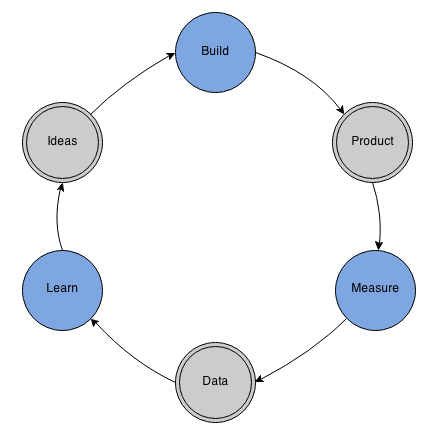
\includegraphics[width=0.5\textwidth]{image/feedback-loop.png}
\end{center}
\caption{Build-Measure-Learn feedback loop}
\label{fig:feedback-loop}
\end{figure}

% -Datan keruu \& oppiminen

~\cite{ries2011lean}

 \subsection{Life Cycle in Lean Startup}

 
 The life cycle in a Lean startup software development doesn't match to the traditional life cycle of a software product. In building a successive product for a software startup, there are usually multiple short iterations surveying the context in which the product will be used. Building a software startup can be started without knowing what the customers want or even who the customers are, so the life cycle of the product has to be built from multiple consecutive version with significant and rapid changes for conforming to the customers demands.

The basic repeating process of development in Lean Startup begins from an idea. This idea contains usually several hypotheses about the customer behavior or the context of usage. Some of these are called leap of faith assumptions, which are the riskiest hypotheses of the plan. Using these hypotheses for validated learning, allows avoiding much of the waste usually present in startups. To utilize the validated learning as a scientific method, there needs to be a selected group of hypotheses to test. The leap of faith assumptions should be the first ones to be tested, because they are the foundation on which the business is to be built. Testing the first hypotheses can be sometimes done with virtually nothing built. This has been done for example by the founder of the online shoe store Zappos, who sold the first pairs of shoes without having any inventory of his own but only some pictures of shoes taken in local shops.

When the first hypotheses have been proved true, hopefully with only a small effort, the Build phase can be initiated and the first Minimum Viable Product (MVP) can be built. This product is a version which enables a full turn of the Build-Measure-Learn loop with minimum effort. This MVP is usually missing most of the features that will be proven essential later. The purpose of this version is that it must be able to measure its impact. The target audience of this product is not the development team or some business heads, but the potential customers, so it can evaluate the reactions of the market.

After the MVP is released, the startup enters the Measure phase. In this phase, the most important topic to get answer for is whether the product development efforts are leading to real progress. In other words: is the product something someone wants. If building something that nobody wants, there is no sense in using time and money on the development. Ries suggests doing the measuring with a method called innovation accounting. It is a quantitative approach for testing if the tuning is successful. It allows creating learning milestones, which are useful for the entrepreneurs for evaluating their progress accurately.

Once the entrepreneurs have learned from the measurements done, it is time for the most important step in the cycle. In this step, the entrepreneurs must assess the success of the hypotheses and based on these assessments, they must decide whether to pivot the original strategy or persevere. If any of the hypotheses proved to be false, it is time for pivot: to make a major change to a new strategic hypothesis. One of the most important objective of the Lean Startup is to allow the recognition of the time to pivot soon, wasting less time and money.

Even though this cycle is called Build-Measure-Learn according to the order of execution, the planning of the cycle is done backwards. The first thing to plan is what is needed to learn. Then using innovation accounting, the things needed to measure are figured out. The last thing is to design the product able to run the experiment returning the measurements.

 Eric Ries reveals multiple success stories using Lean Startup, in where there are many similarities. One of the success stories is about a collaboration portal for voters. The first released version of the portal was achieved with 1200\$ and three months of work. With that version, some of the assumptions could be tested in the real operating environment and the product could be developed further. After the partial success of the first version, there were five other version of the portal and the business model developed. After each of the launches, the leaps of faith were tested and the necessary changes were made for steering the product to the right direction. After 16 months of development the product had reached a sufficient state for a sustainable business. During these months, there had been several pivots and changes, which cannot be seen as a traditional product life cycle.



% Tässä scopessa ei perinteisessä mielessä life cycleä
% Iteratiivista kehitystä, MVP, continuous deploymentia ja pivoteja
% http://blogs-images.forbes.com/martinzwilling/files/2013/02/valley-of-death.jpg
% Votizen p.150
%	-5 MVP:tä 

% \begin{itemize}

% \item Startup financing cycle (Valley of Death)
% \item Iteratiivinen kehitys
% \item Lyhyet sprintit
 
% \end{itemize}
 
% \subsection{Product scope}
 
%PMBOK p. 51 Project scope management
%	-Product scope
%	-Project scope


% \begin{itemize}
 
% \item Analytics
% \item Ominaisuuksien priorisointi (esim. käytön mukaan)
% \item Scope
% \item MVP
% \item Valitaan oikeat feature
% \item Validoinnit: I Know I When I See It
% \item Leanista jotain tännekin
 
% \end{itemize}
 

%%%%%%%%%%%%%%%%%%%%%%%%%%%%%%%%%%%%%%%%%%%%%%%%%%%%%%%%%%%%%%%%%%%%%%%%%%%%%%%%%%%%%%%%%%%%%%%
%	REFERENCES
%%%%%%%%%%%%%%%%%%%%%%%%%%%%%%%%%%%%%%%%%%%%%%%%%%%%%%%%%%%%%%%%%%%%%%%%%%%%%%%%%%%%%%%%%%%%%%%


% lähdeluettelo
% seuraavia voi käyttää bibtex:n kanssa (edellyttää tiedoston books.bib)
\bibliographystyle{plain}
\bibliography{books}
 
%\appendix
%\renewcommand{\chaptername}{Liite}

 
%\chapter{Liitteitä}
\end{document}
